% THIS IS SIGPROC-SP.TEX - VERSION 3.1
% WORKS WITH V3.2SP OF ACM_PROC_ARTICLE-SP.CLS
% APRIL 2009
%
% It is an example file showing how to use the 'acm_proc_article-sp.cls' V3.2SP
% LaTeX2e document class file for Conference Proceedings submissions.
% ----------------------------------------------------------------------------------------------------------------
% This .tex file (and associated .cls V3.2SP) *DOES NOT* produce:
%       1) The Permission Statement
%       2) The Conference (location) Info information
%       3) The Copyright Line with ACM data
%       4) Page numbering
% ---------------------------------------------------------------------------------------------------------------
% It is an example which *does* use the .bib file (from which the .bbl file
% is produced).
% REMEMBER HOWEVER: After having produced the .bbl file,
% and prior to final submission,
% you need to 'insert'  your .bbl file into your source .tex file so as to provide
% ONE 'self-contained' source file.
%
% Questions regarding SIGS should be sent to
% Adrienne Griscti ---> griscti@acm.org
%
% Questions/suggestions regarding the guidelines, .tex and .cls files, etc. to
% Gerald Murray ---> murray@hq.acm.org
%
% For tracking purposes - this is V3.1SP - APRIL 2009

\documentclass{acm_proc_article-sp}
\usepackage{amsmath}
\usepackage{url}
\usepackage{graphicx}
\usepackage{alltt}
\usepackage{algorithm}

\usepackage{algorithmic}
\usepackage{cite}
\usepackage{flushend}
\usepackage{tabularx}
\usepackage{framed}

%\lstset{language=C}
\usepackage{times}
\usepackage{graphicx}
\usepackage{epsf}
\usepackage{verbatim}
\usepackage{psfig}
\usepackage{cite}
\usepackage{url}
\usepackage{color}
\usepackage[table]{xcolor}
\usepackage{booktabs, dcolumn}
\usepackage{alltt}

\usepackage{longtable,lscape}
\usepackage{slashbox,multirow}
\usepackage{colortbl}
\usepackage{mathrsfs}

\newcommand{\Add}{\CodeIn{add}}
\newcommand{\AVTree}{\CodeIn{AVTree}}
\newcommand{\Assignment}[3]{$\langle$ \Object{#1}, \Object{#2}, \Object{#3} $\rangle$}
\newcommand{\BinaryTreeRemove}{\CodeIn{BinaryTree\_remove}}
\newcommand{\BinaryTree}{\CodeIn{BinaryTree}}
\newcommand{\Caption}{\caption}
\newcommand{\Char}[1]{`#1'}
\newcommand{\CheckRep}{\CodeIn{checkRep}}
\newcommand{\ClassC}{\CodeIn{C}}
\newcommand{\CodeIn}[1]{{\small\texttt{#1}}}
\newcommand{\CodeOutSize}{\scriptsize}
\newcommand{\Comment}[1]{}
\newcommand{\Ensures}{\CodeIn{ensures}}
\newcommand{\ExtractMax}{\CodeIn{extractMax}}
\newcommand{\FAL}{field-ordering}
\newcommand{\FALs}{field-orderings}
\newcommand{\Fact}{observation}
\newcommand{\Get}{\CodeIn{get}}
\newcommand{\HashSet}{\CodeIn{HashSet}}
\newcommand{\HeapArray}{\CodeIn{HeapArray}}
\newcommand{\Intro}[1]{\emph{#1}}
\newcommand{\Invariant}{\CodeIn{invariant}}
\newcommand{\JUC}{\CodeIn{java.\-util.\-Collections}}
\newcommand{\JUS}{\CodeIn{java.\-util.\-Set}}
\newcommand{\JUTM}{\CodeIn{java.\-util.\-TreeMap}}
\newcommand{\JUTS}{\CodeIn{java.\-util.\-TreeSet}}
\newcommand{\JUV}{\CodeIn{java.\-util.\-Vector}}
\newcommand{\JMLPlusJUnit}{JML+JUnit}
\newcommand{\Korat}{Korat}
\newcommand{\Left}{\CodeIn{left}}
\newcommand{\Lookup}{\CodeIn{lookup}}
\newcommand{\MethM}{\CodeIn{m}}
\newcommand{\Node}[1]{\CodeIn{N}$_#1$}
\newcommand{\Null}{\CodeIn{null}}
\newcommand{\Object}[1]{\CodeIn{o}\ensuremath{_#1}}
\newcommand{\PostM}{\MethM$_{post}$}
\newcommand{\PreM}{\MethM$_{pre}$}
\newcommand{\Put}{\CodeIn{put}}
\newcommand{\Remove}{\CodeIn{remove}}
\newcommand{\RepOk}{\CodeIn{repOk}}
\newcommand{\Requires}{\CodeIn{requires}}
\newcommand{\Reverse}{\CodeIn{reverse}}
\newcommand{\Right}{\CodeIn{right}}
\newcommand{\Root}{\CodeIn{root}}
\newcommand{\Set}{\CodeIn{set}}
\newcommand{\State}[1]{2^{#1}}
\newcommand{\TestEra}{TestEra}
\newcommand{\TreeMap}{\CodeIn{TreeMap}}

\newenvironment{CodeOut}{\begin{scriptsize}}{\end{scriptsize}}
\newenvironment{SmallOut}{\begin{small}}{\end{small}}

\newcommand{\pairwiseEquals}{PairwiseEquals}
\newcommand{\monitorEquals}{MonitorEquals}
%\newcommand{\monitorWField}{WholeStateW}
\newcommand{\traverseField}{WholeState}
\newcommand{\monitorSMSeq}{ModifyingSeq}
\newcommand{\monitorSeq}{WholeSeq}

\newcommand{\IntStack}{\CodeIn{IntStack}}
\newcommand{\UBStack}{\CodeIn{UBStack}}
\newcommand{\BSet}{\CodeIn{BSet}}
\newcommand{\BBag}{\CodeIn{BBag}}
\newcommand{\ShoppingCart}{\CodeIn{ShoppingCart}}
\newcommand{\BankAccount}{\CodeIn{BankAccount}}
\newcommand{\BinarySearchTree}{\CodeIn{BinarySearchTree}}
\newcommand{\LinkedList}{\CodeIn{LinkedList}}

\newcommand{\Book}{\CodeIn{Book}}
\newcommand{\Library}{\CodeIn{Library}}

\newcommand{\Jtest}{Jtest}
\newcommand{\JCrasher}{JCrasher}
\newcommand{\Daikon}{Daikon}
\newcommand{\JUnit}{JUnit}

\newcommand{\trie}{trie}

\newcommand{\Perl}{Perl}


\newcommand{\SubjectCount}{11}
\newcommand{\DSSubjectCount}{two}

\newcommand{\Equals}{\CodeIn{equals}}
\newcommand{\Pairwise}{PairwiseEquals}
\newcommand{\Subgraph}{MonitorEquals}
\newcommand{\Concrete}{WholeState}
\newcommand{\ModSeq}{ModifyingSeq}
\newcommand{\Seq}{WholeSeq}
\newcommand{\Aeq}{equality}

\newcommand{\Meaning}[1]{\ensuremath{[\![}#1\ensuremath{]\!]}}
\newcommand{\Pair}[2]{\ensuremath{\langle #1, #2 \rangle}}
\newcommand{\Triple}[3]{\ensuremath{\langle #1, #2, #3 \rangle}}
\newcommand{\SetSuch}[2]{\ensuremath{\{ #1 | #2 \}}}

\newcommand{\Equiv}[2]{\ensuremath{#1 \EquivSTRel{} #2}}
\newcommand{\EquivME}{\Equiv}
\newcommand{\EquivST}{\Equiv}
\newcommand{\EquivSTRel}{\ensuremath{\cong}}
\newcommand{\Redundant}[2]{\ensuremath{#1 \lhd #2}}
\newcommand{\VB}{\ensuremath{\mid}}
\newcommand{\MES}{method-entry state}

\newcommand{\Small}[1]{{\small{#1}}}

\newcommand{\CenterCell}[1]{\multicolumn{1}{c|}{#1}}

% Yoonki's code
\colorlet{tableheadcolor}{gray!15} % Table header colour = 25% gray
\newcommand{\headcol}{\rowcolor{tableheadcolor}} %
\colorlet{tablerowcolor}{gray!5} % Table row separator colour = 10% gray
\colorlet{tablerowcolor2}{gray!0}
\newcommand{\rowcol}{\rowcolor{tablerowcolor}} %
\newcommand{\rowpln}{\rowcolor{tablerowcolor2}} %
    % Command \topline consists of a (slightly modified) \toprule followed by a \heavyrule rule of colour tableheadcolor (hence, 2 separate rules)
\newcommand{\topline}{\arrayrulecolor{black}\specialrule{0.1em}{\abovetopsep}{0pt}%
            \arrayrulecolor{tableheadcolor}\specialrule{\belowrulesep}{0pt}{0pt}%
            \arrayrulecolor{black}}
    % Command \midline consists of 3 rules (top colour tableheadcolor, middle colour black, bottom colour white)
\newcommand{\midline}{\arrayrulecolor{tableheadcolor}\specialrule{\aboverulesep}{0pt}{0pt}%
            \arrayrulecolor{black}\specialrule{\lightrulewidth}{0pt}{0pt}%
            \arrayrulecolor{white}\specialrule{\belowrulesep}{0pt}{0pt}%
            \arrayrulecolor{black}}
    % Command \rowmidlinecw consists of 3 rules (top colour tablerowcolor, middle colour black, bottom colour white)
\newcommand{\rowmidlinecw}{\arrayrulecolor{tablerowcolor}\specialrule{\aboverulesep}{0pt}{0pt}%
            \arrayrulecolor{black}\specialrule{\lightrulewidth}{0pt}{0pt}%
            \arrayrulecolor{white}\specialrule{\belowrulesep}{0pt}{0pt}%
            \arrayrulecolor{black}}
    % Command \rowmidlinewc consists of 3 rules (top colour white, middle colour black, bottom colour tablerowcolor)
\newcommand{\rowmidlinewc}{\arrayrulecolor{white}\specialrule{\aboverulesep}{0pt}{0pt}%
            \arrayrulecolor{black}\specialrule{\lightrulewidth}{0pt}{0pt}%
            \arrayrulecolor{tablerowcolor}\specialrule{\belowrulesep}{0pt}{0pt}%
            \arrayrulecolor{black}}
    % Command \rowmidlinew consists of 1 white rule
\newcommand{\rowmidlinew}{\arrayrulecolor{white}\specialrule{\aboverulesep}{0pt}{0pt}%
            \arrayrulecolor{black}}
    % Command \rowmidlinec consists of 1 tablerowcolor rule
\newcommand{\rowmidlinec}{\arrayrulecolor{tablerowcolor}\specialrule{\aboverulesep}{0pt}{0pt}%
            \arrayrulecolor{black}}
    % Command \bottomline consists of 2 rules (top colour
\newcommand{\bottomline}{\arrayrulecolor{white}\specialrule{\aboverulesep}{0pt}{0pt}%
            \arrayrulecolor{black}\specialrule{\heavyrulewidth}{0pt}{\belowbottomsep}}%
\newcommand{\bottomlinec}{\arrayrulecolor{tablerowcolor}\specialrule{\aboverulesep}{0pt}{0pt}%
            \arrayrulecolor{black}\specialrule{\heavyrulewidth}{0pt}{\belowbottomsep}}%

%\usepackage[margin=0.5in]{geometry}

\begin{document}

\title{Discovering Likely Mappings between APIs using Text Mining}
%\subtitle{[Extended Abstract]
%\titlenote{A full version of this paper is available as
%\textit{Author's Guide to Preparing ACM SIG Proceedings Using
%\LaTeX$2_\epsilon$\ and BibTeX} at
%\texttt{www.acm.org/eaddress.htm}}}
%
% You need the command \numberofauthors to handle the 'placement
% and alignment' of the authors beneath the title.
%
% For aesthetic reasons, we recommend 'three authors at a time'
% i.e. three 'name/affiliation blocks' be placed beneath the title.
%
% NOTE: You are NOT restricted in how many 'rows' of
% "name/affiliations" may appear. We just ask that you restrict
% the number of 'columns' to three.
%
% Because of the available 'opening page real-estate'
% we ask you to refrain from putting more than six authors
% (two rows with three columns) beneath the article title.
% More than six makes the first-page appear very cluttered indeed.
%
% Use the \alignauthor commands to handle the names
% and affiliations for an 'aesthetic maximum' of six authors.
% Add names, affiliations, addresses for
% the seventh etc. author(s) as the argument for the
% \additionalauthors command.
% These 'additional authors' will be output/set for you
% without further effort on your part as the last section in
% the body of your article BEFORE References or any Appendices.

\numberofauthors{1} %  in this sample file, there are a *total*
% of EIGHT authors. SIX appear on the 'first-page' (for formatting
% reasons) and the remaining two appear in the \additionalauthors section.
%
\author{
% You can go ahead and credit any number of authors here,
% e.g. one 'row of three' or two rows (consisting of one row of three
% and a second row of one, two or three).
%
% The command \alignauthor (no curly braces needed) should
% precede each author name, affiliation/snail-mail address and
% e-mail address. Additionally, tag each line of
% affiliation/address with \affaddr, and tag the
% e-mail address with \email.
%
% 1st. author
\alignauthor
{\large Rahul Pandita$^\dagger$, Raoul Praful Jetley$^\mp$, Sithu D Sudarsan$^\mp$, and Laurie Williams$^\dagger$}\\%\titlenote{Dr.~Trovato insisted his name be first.}\\
\affaddr{$^\dagger$North Carolina State University, Raleigh, NC, USA}\\
\affaddr{$^\mp$ABB Corporate Research, Bangalore, India}\\
\email{{\normalsize rpandit@ncsu.edu, raoul.jetley@in.abb.com, sudarsan.sd@in.abb.com, williams@csc.ncsu.edu}}
}


\date{30 July 1999}
% Just remember to make sure that the TOTAL number of authors
% is the number that will appear on the first page PLUS the
% number that will appear in the \additionalauthors section.

\maketitle

\newcommand{\tool}{{\sc TMAP}}
\begin{abstract}

Developers often migrate their applications to support various platform/programming-language application programming interfaces (APIs) to retain existing users and to attract new users.
For example, a typical mobile software developer releases his/her applications
on all the popular mobile platforms, such as Android, iOS, and Windows.
To migrate an application written using one API (source) to another API (target), a developer must know how the methods in the source API map to the methods in the target API.
Given a typical platform or language exposes a large number of API methods, manually discovering API mappings is prohibitively resource-intensive and may be error prone.
\textit{The goal of this research is to support software developers 
	in migrating an application from a source API to a target API
	by automatically discovering relevant method mappings across APIs using text mining
	on the natural language API method descriptions.}
This paper proposes \tool: \textbf{T}ext \textbf{M}ining based approach to discover relevant \textbf{AP}I mappings.
Since, \tool\ uses as input the natural language text in API documents instead of source code,
our approach compliments existing program-analysis based approaches such as Rosetta and StaMiner
that require as input a manually ported software or at least functionally similar software across source and target APIs to find method mappings.
To evaluate our approach, we used \tool\ to discover API mappings for 15 classes across: 
 1) \CodeIn{Java} and \CodeIn{C\#} API; and
 2) \CodeIn{Java ME} and \CodeIn{Android} API.
 We compared the discovered mappings with state-of-the-art source code analysis-based approaches: Rosetta and StaMiner.
 Furthermore, our results also show promise in leveraging user feedback to prune irrelevant suggestions in the \tool\ output.
\end{abstract}


% A category with the (minimum) three required fields
%\category{H.4}{Information Systems Applications}{Miscellaneous}
%A category including the fourth, optional field follows...
\category{D.2.7}{Software Engineering}{Distribution, Maintenance, and Enhancement}[Documentation, Restructuring, reverse engineering, and reengineering]


%\terms{Theory}

\keywords{API documents, text mining} % NOT required for Proceedings

\section{Introduction}
\label{sec:introduction}

%For instance, a typical user may view emails on his/her Android or iOS or WindowsPhone handheld
%device, such as a mobile phone or a tablet. 
%The user then can switch to a desktop environment, such as Windows or Linux or OSX 
%in an workplace like setting through either a web browser or 
%a standalone application, such as Microsoft Outlook or Mozilla Thunderbird.

Developers are increasingly releasing different versions of their applications to attract new users and to retain existing users across different platforms.
For example, a typical mobile software developer often releases his/her applications
on all the popular mobile platforms, such as Android, iOS, and Windows,
which often involves rewriting applications in different languages.
For instance, Java is the preferred language for implementing Android applications
and Swift for iOS applications.
In the context of desktop software, many well-known projects, such as JUnit and
Hibernate, provide multiple versions in different programming languages
to attract the developer community to use these
libraries across those languages.


%However, manually migrating a software from one platform (/language) to another
%can be time consuming and may be error prone.

Existing tools, such as Java2CSTranslator~\cite{java2cstranslator},
assist developers by automating the process of software migration.
However, such tools require a programmer to manually input
how methods in a source language's Application Programming Interfaces (API) maps to the methods of the target language's API. 
Given a typical language (or platform) exposes a large number of API methods for developers to reuse, manually discovering these mappings is prohibitively resource intensive and may be error prone.


Existing program analysis-based approaches
address the problem of finding method mappings between APIs using
static~\cite{Zhong2010ICSE} and dynamic~\cite{Gokhale2013ICSE} analysis. 
Recently, Nguyen et al.~\cite{nguyen2014statistical} further proposed to
apply statistical language translation techniques to achieve language migration
by mining large corpora of open source software repositories.
However, these approaches require as an input manually-ported software
or at least functionally-similar software artrifcats(source-code or binaries)
across source and target APIs.
Since static analysis approaches~\cite{Zhong2010ICSE,nguyen2014statistical}
leverage source code analysis, 
accuracy of such approaches is dependent on the quality of the code under consideration.
Likewise, accuracy of dynamic approaches~\cite{Gokhale2013ICSE} is dependent on
the quality and completeness of test inputs
to exercise the API behavior comprehensively. 
Furthermore, such program analysis approaches are often sensitive to the nuances of
the programming language of the source code under analysis, thus require significant effort
for accommodating new programming languages.  


\textit{The goal of this research is to support software developers 
	in migrating an application from a source API to a target API
	by automatically discovering relevant method mappings across APIs using text mining
	on the natural language API method descriptions.}

We propose to use the natural language API method descriptions
to discover the method mappings across APIs.
We hypothesize:
\textit{since the API documents are targeted towards developers,
	there may be an overlap in the language used to describe similar concepts that can be leveraged.}
In general, API documentation provides developers with useful information
about class/interface hierarchies within the software.
Additionally, API documents also provide information about
how to use a particular method within a class by means of method descriptions.
A method description typically outlines specifications in terms of
the expectations of the method arguments and functionality of method in general.


This paper presents \tool : An approach that leverages the natural language method descriptions to discover the likely method mapping between APIs.
\tool\ stands for \textit{\textbf{T}ext \textbf{M}ining
	based approach to discover likely \textbf{AP}I method mappings}.
\tool\ accepts as input the API doucments of source and target API.
In particular, \tool\ proposes to create a vector space model~\cite{singhal2001modern,manning2008introduction} of the target API method descriptions. 
\tool\ then queries the vector space model of the target API using
automatically-generated queries from the source API method descriptions.
\tool\ automates the query generation in source API using the concepts from text mining, such as emphasizing certain keywords over others and querying multiple facets of API documents, such as class description, package names, and method description.
The output of \tool\ is a ranked list of methods of the target API that are candidates for the mapping of the method from the source API that was used to generate the query.
Since \tool\ analyzes API documents in natural language, the proposed approach is reusable, independent of the programming language of the library.


However, automatic query generation is challenging. In particular, given a typical API exposes a large number of methods, a large search space may result in noise in the search results.
Consider for example, Android API level 23 exposes 4404~\footnote{\url{http://developer.android.com/reference/classes.html}} classes
and Java 8 exposes 4240~\footnote{\url{https://docs.oracle.com/javase/8/docs/api/allclasses-noframe.html}} classes.
Furthermore, each class exposes several methods resulting in a large search space for each query and a low effectiveness of search. 
\tool\ addresses this challenge by leveraging feedback in the form of confirmed mappings to prune the search space using topic modelling~\cite{blei2003latent,panichella2013effectively}.
Thus, given a set of confirmed mappings \tool\ improves the recommendations for future queries by pruning irrelevant methods from search results.


We pose the following research questions:
\begin{itemize}
	
	\item\textbf{RQ1}: Does \tool\ discover additional method mappings in comparison to existing program-analysis based approaches?
	
	\item\textbf{RQ2}: What is the improvement in pruning irrelevant mappings from the \tool\ output by leveraging feedback?
	
	\item\textbf{RQ3}: What is the overlap of the method mappings discovered by \tool\ in comparison with the mappings discovered by existing program-analysis based approaches?
	
	
	\item\textbf{RQ4}: Does \tool\ discover relevant methods using free-form queries instead of automatically generated queries?
	
\end{itemize}
To answer our questions, we apply \tool\ to discover likely API mappings for 15 classes across:
1) \CodeIn{Java} and \CodeIn{C\#} API; and 2) \CodeIn{Java ME}~\footnote{Java Platform Micro Edition} and \CodeIn{Android} API.
We also compare the discovered mappings with two state-of-the-art program-analysis based approaches: Rosetta~\cite{Gokhale2013ICSE} and StaMiner~\cite{nguyen2014statistical}.
%Our results indicate that \tool\ on an average found relevant mappings for 57\% more methods compared to Rosetta and StaMiner. 
%Furthermore, our results also indicate that \tool\ found on average exact mappings for 6.5 more methods per class with a maximum of 21 additional exact mappings for a single class as compared to previous approaches.

%In summary, \tool\ leverages natural language description of APIs to discover likely mapping thus facilitating cross API migration of applications. Since \tool\ analyzes API documents in natural language, the proposed approach is reusable, independent of the programming language of the library. 

This paper makes the following major contributions:
\begin{itemize}
	\item A text mining (queries on vector space model) based approach that effectively discovers mapping between source and target API.
	\item A topic modeling-based feedback approach for reducing the search space of queries to prune irrelevant suggestions in discovering mapping between source and target API. 
	\item A prototype implementation of our approach based on extending the Apache Lucene~\cite{lucene} and Mallet~\cite{McCallum}. An open source implementation of our prototype can be found at our website~\cite{projectWeb}. 
	\item An evaluation of our approach on 5 classes in Java ME to Android API and 10 Classes Java to C\# API. The evaluation results and artifacts are publicly available on the project website.
\end{itemize}


This paper is a revised, expanded version of a paper (Pandita et al.~\cite{pandita2015discovering}) presented at the 15th
IEEE working conference on Source Code Analysis and Maintenance (SCAM 2015).
Specifically, this paper builds on the previous version by proposing and evaluating a new technique to leverage feedback for prune the irrelevant \tool\ suggestions. Furthermore, this paper also evaluates the effectiveness of text-mining in general for API related information retrieval tasks.

The rest of the paper is organized as follows.
Section~\ref{sec:background} presents the background on Text Mining.
Section~\ref{sec:example} presents a real world example that motivates our approach. Section~\ref{sec:approach} presents \tool\ approach.
Section~\ref{sec:evaluation} presents evaluation of \tool.
Section~\ref{sec:discussion} presents a brief discussion and future work.
Section~\ref{sec:related} discusses the related work.
Finally, Section~\ref{sec:conclusion} concludes the paper.


\vspace*{-1ex}
\section{Background}
\label{sec:background}
\vspace*{-1ex}

Text mining is a broad research area, 
including but not limited to the techniques 
facilitating retrieval/manipulation of useful information from a large corpus to text. 
%A recent study~\cite{russom2011big} indicates that 
%a significant (35\%) of business information is captured in unstructured data.
%A large part of this information is in 
%documents containing narrative text, such as reports,
%presentations, web data, and design documents.
%Text mining is used to infer the knowledge
%in these documents through a combination of extraction and analytical methods. 
As opposed to traditional data mining, text mining analyzes
free-form text distributed across documents
(rather than data localized and maintained within a database).
To analyze this data, text mining uses concepts from traditional
data analytics, natural language processing, and data modeling.
We next introduce the concepts from text mining that have been used in the presented approach.


\textbf{Indexing}~\cite{frakes1992introduction,manning2008introduction}:
Indexing is the process of extracting text data from source documents
and storing them in well-defined indexes.
During the indexing process, a document (a sequence of text) is divided into its constituent units, known as tokens or terms, based on a well-defined criterion. 
A term is typically an individually identifiable unit of the document (such as a word) and relates to the individual terms stored in an index. Once the terms within each document are identified, they are added to the index, with the corresponding link to the document and associated term frequencies.
Term frequency is the simple count of the occurrence of a term in a document.
An optional pre-processing step further assists with indexing, such as removing stop-words. 

%However, simply adding all identified tokens to the index can introduce a number of inefficiencies, primarily because of the commonly used terms (like articles, prepositions, conjunctions, etc.), which not only bloat the index, but can also adversely affect the search/retrieval results. To avoid this, a common strategy is to clean the tokens to eliminate unwanted words before populating the index. Another pre-processing strategy that is commonly employed is to group together similar words (based on their meanings) to provide a semantic search capability and improve the hit rate when searching for related terms.\textbf{Describe attribute definition}

Among various indexing strategies,
the use of \textit{inverted file indexing}~\cite{frakes1992introduction}
is well suited for large document collections.
In the simplest form, an inverted file index provides
a mapping of terms, such as words, to its locations in a text document.
A document can be thought of as a collection of $m$ terms.
Typically a document is made up of a sequence of $n$ unique terms
such that $n <= m$.
The number n is usually far less than
$m$ as most of the terms are repeated while forming a document. 
For instance, the term ``the'' is repeated many times in this paper.
The set of unique terms within an index forms
the ``Term List'' $v$ of the index.
If a pointer (say numeric location) is associated with each term in $v$ to the location
of that term in text document, the resultant data structure
is a form of inverted file index.
As the document collection grows,
the number of documents matching a term in the index becomes sparser.

The index is oftentimes annotated with the information regarding 
the frequency of occurrence of each term in the document. 
The representation of a document as a vector of frequencies
of terms is referred to as \textit{vector space model}~\cite{singhal2001modern,frakes1992introduction}.

\textbf{TF-IDF}\cite{manning2008introduction}:
Term -frequency inverse-document-frequency (\CodeIn{tf-idf}) is a numerical statistic that is intended to capture the importance of a term to a document in a corpus.
Often used as a weighting metric in information retrieval and text mining,
the \CodeIn{tf-idf} weight increases proportionally to frequency of the occurrence of a term in a document; however, the weight is also offset by the count of the number of documents that contain the term.

\textbf{Cosine Similarity}\cite{singhal2001modern}: In mathematics, Cosine similarity is a numerical statistic to measure the similarity between two vectors.
Cosine similarity is defined as a dot product of magnitude of two vectors.
In context of text mining, the Cosine similarity is used to capture the similarity between two documents represented as term frequency vectors.

%\textbf{Topic Modelling}: Latent Drichilet Allocation (LDA)~\cite{blei2003latent,panichella2013effectively} is an Information Retrieval (IR) 
%model to fit a probabilistic model on the term occurrences in a corpus of documents.
%Given a corpus of $n$ documents, a dictionary is created.
%The dictionary consists a list of all the unique terms ($m$) occurring in all $n$ documents.
%Next, a term-to-document matrix $M$ of size $(m\ X\ n)$ is generated, where each row represents all the terms occurring the corpus and columns representing the all the documents in the corpus.
%Each cell of $M$ ($M[i,j]$) contains the weight of the $i^{th}$ term in $m$ in the $j^{th}$ document in $n$.
%In the simplest implementation \CodeIn{tf-idf} is used to calculate the weight of a term in a document.
%
%
%Next LDA transforms term-to-document matrix $M$ into a topic-to-document matrix $\theta$ of size $(k\ X\ n)$,
%where each row represents the topics occurring in the corpus and columns representing the all the documents in the corpus. 
%This transformation is achieved by identifying latent variables (topics) in the documents. 
%The parameter $k$ is independently provided as an argument to the LDA algorithm.
%Each cell of $\theta\ (\theta[i,j])$ contains the probability of the $i^{th}$ topic in $k$ occurring in the $j^{th}$ document in $n$. Since $k\ <<\ m$, LDA is a mapping of the documents from the term space $m$ to the topic space $k$~\cite{panichella2013effectively}.
%
%
%\begin{enumerate}
%	\item $k$, the total number of topics to be extracted from a corpus of documents.
%	\item $n$, the total number of gibbs iteration, where a single iteration involves a gibbs sampler sampling a topic for each term occurring in the corpus.
%	\item $\alpha$, this parameter affects the distribution of topics across documents. A high $\alpha$ means that each document is likely to contain a mixture of most of the topics. Conversely, a low $\alpha$ means each document is likely to contain mixture of fewer or one topic. 
%	\item $\beta$, this parameter affects the distribution of terms in each topic. A high $\beta$ means that each topic is likely to contain a uniform distribution of terms. Conversely, a low $\beta$ means terms are not uniformly distributed across topics. 
%	
%\end{enumerate}
\section{Examples}
\label{sec:example}

We now present a series progressing in complexity to demonstrate our approach. Our examples are from real Java Platform, Micro Edition (JME) formerly known as J2ME and Android API. Both JME and Android use Java as the language of implementation and targeted towards hand-held devices. However, our approach is independent of language of implementation and thus can be used for any similar source and target API.  

First we parse the API documents of source and target API library and store it in intermediate representation for analysis. In particular, we extract class, interface and corresponding method descriptions from API documents. Second, we then create a term vector representation of each class description and method descriptions. Vector space model or term vector model is an algebraic model for representing text documents (and any objects, in general) as vectors of identifiers, such as, for example, index terms. In our case, each word is considered as a term barring the stop words such as (a, the, and ...). 

Finally we use the term vector representation of a method description in a source API to query term vector representation of the the method description in target API. The results are ranked based on the Term Frequency-Inverse Document Frequency (TF-IDF) measure. TF-IDF is a numerical statistic which reflects how important a word is to a document in a collection or corpus. It is often used as a weighting factor in information retrieval and text mining.

We then collect the top 10 results from target API methods for each source API method. Figure~\ref{fig:excpAPIJ2ME} and Figure~\ref{fig:excpAPIAndroid} shows example of trivially similar API methods. Our search results return the Android API method shown in Figure~\ref{fig:excpAPIAndroid} as a first match for the JME method shown in Figure~\ref{fig:excpAPIJ2ME}. Notice the slightly different description for the methods in JME and Android API. Although, correct this is very trivial mapping. We next present a more complex example.  

\begin{figure}[t]
\begin{CodeOut}
\begin{alltt}
\includegraphics[scale=0.45]{AritmeticExceptionJ2ME.eps}
\end{alltt}
\end{CodeOut}
\caption{\label{fig:excpAPIJ2ME} The method description of the \CodeIn{ArithmeticException} method in J2ME API}
\end{figure}



\begin{figure}[t]
\begin{CodeOut}
\begin{alltt}
\includegraphics[scale=0.45]{AritmeticExceptionAndroid.eps}
\end{alltt}
\end{CodeOut}
\caption{\label{fig:excpAPIAndroid} The method description of the \CodeIn{ArithmeticException} method in Android API}
\end{figure}

Figure~\ref{fig:drawCharAPIJ2ME} and Figure~\ref{fig:drawTextAPIJ2ME} shows example of non-trivially similar API methods. Although, the textual description is similar using text analytics (TF-IDF similarity using term frequency vector), there is difference in type of arguments.

Our approach first tries to align the arguments:
\begin{enumerate}
\item int is matched to float common knowledge
\item \CodeIn{Type} analysis for \CodeIn{Paint} is performed to get additional (previous) method invocations
\item \CodeIn{Type} analysis of \CodeIn{Anchor} is performed to get additional method invocations
\end{enumerate}



\begin{figure}[t]
\begin{CodeOut}
\begin{alltt}
\includegraphics[scale=0.45]{drawStringJ2ME.eps}
\end{alltt}
\end{CodeOut}
\caption{\label{fig:drawCharAPIJ2ME} The method description of the \CodeIn{drawChar} method in J2ME API}
\end{figure}

\begin{figure}[t]
\begin{CodeOut}
\begin{alltt}
\includegraphics[scale=0.45]{drawTextAndroid.eps}
\end{alltt}
\end{CodeOut}
\caption{\label{fig:drawTextAPIJ2ME} The method description of the \CodeIn{drawText} method in Android API}
\end{figure}
\vspace*{-1ex}
\section{Approach}
\label{sec:approach}
\vspace*{-1ex}

We next present our approach for discovering 
likely mappings of API methods  across APIs. 
Figure~\ref{fig:approachOverview} provides an overview of the \tool\ approach.
The \tool\ approach consists of three major components: 1) an Indexer; 2) Query Builder; and 3) Searcher components.


The Indexer accepts the API documents of the target API
and creates indexes (a vector space model) of these documents 
by extracting intermediate contents from the method descriptions. 
The Query Builder accepts the API documents of the source API
and creates queries to be executed on the indexes (a vector space model).
Finally, Searcher component executes the queries on the indexes and 
generates a ranked list of the API methods from target API documents as
mapping results to be presented to the developers for confirmation. 
We next describe each component in detail.


\begin{figure}
	\begin{center}
		%\begin{framed}
		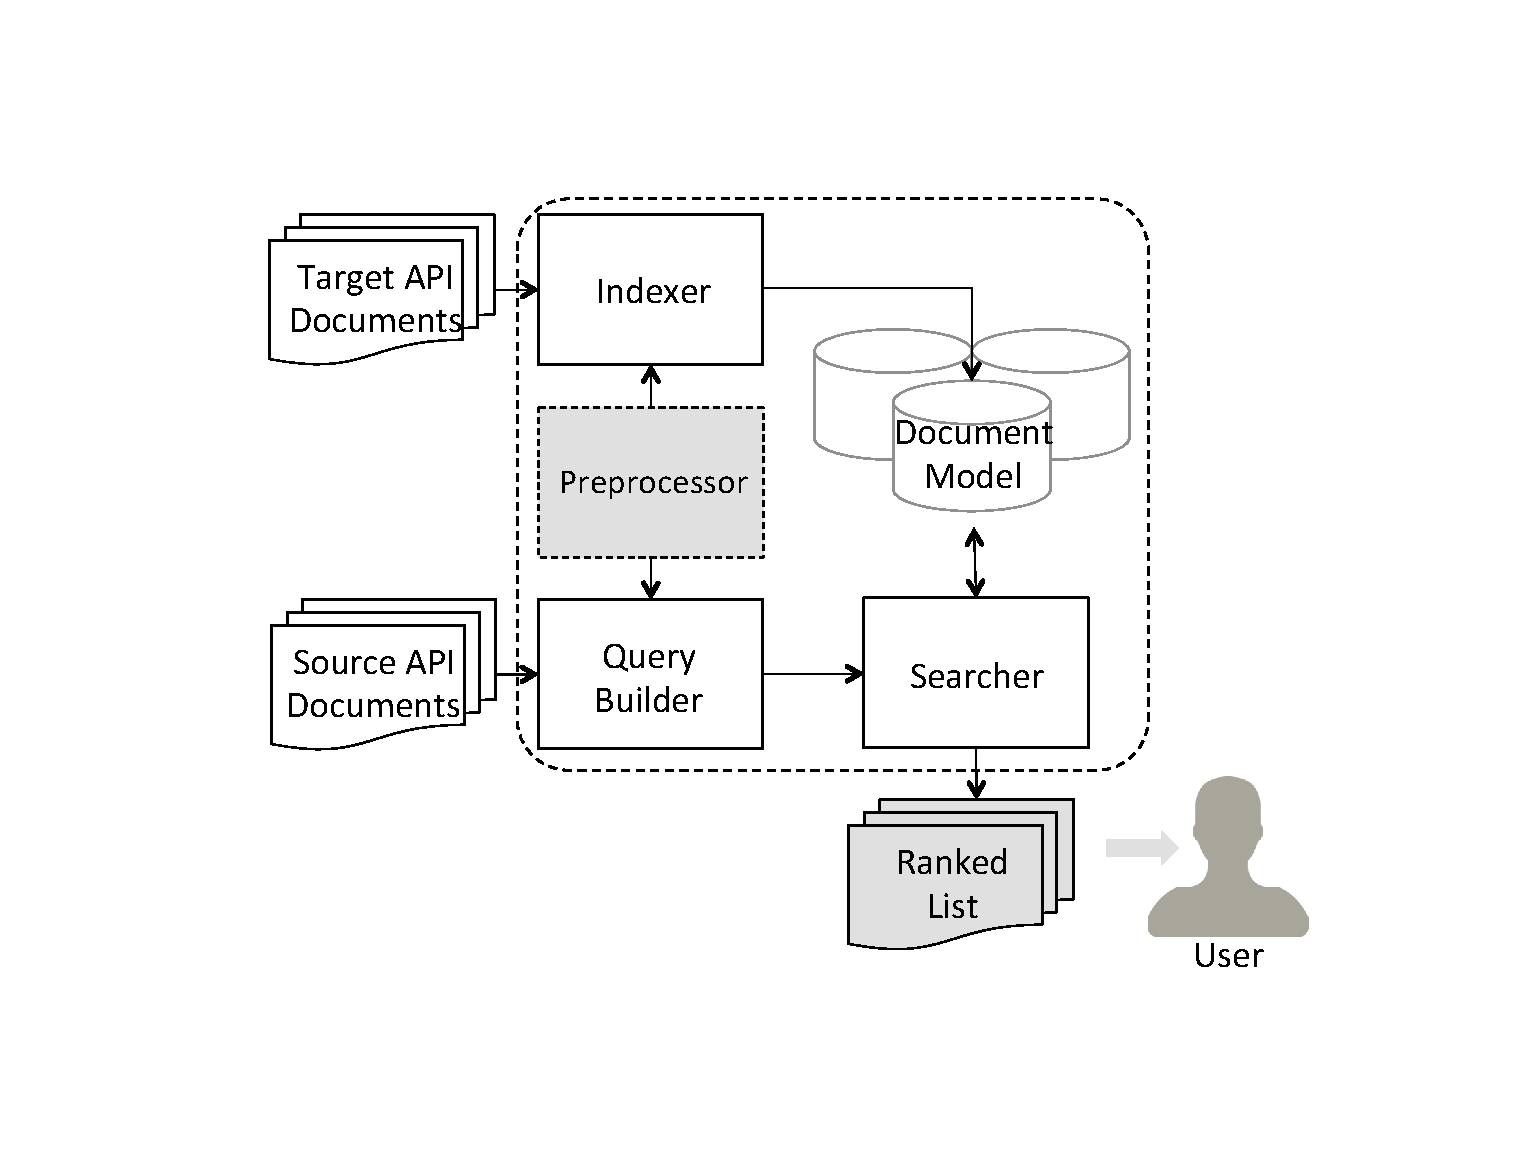
\includegraphics[scale=0.45,clip=true, trim=120pt 80pt 10pt 80pt]{ApproahOverview.eps}
		%\end{framed}
		\vspace*{-4ex}
		\caption{\label{fig:approachOverview} Overview of \tool\ approach}
	\end{center}
	\vspace*{-4ex}
\end{figure}


\subsection{Indexer}
\label{sub:Approach_Indexer}

This component accepts the API method descriptions of the target API
and creates indexes (a vector space model) of these documents.
In particular, Indexer extracts the following fields from the API method descriptions:

 
\textbf{F1) Type Name}: The name of enclosing class/interface of the method. For the method description of \CodeIn{drawString} shown in Figure~\ref{fig:drawStringJavadoc}, indexer extracts the type Name as ``Graphics''.
	
\textbf{F2) Package Name}: The package name of the enclosing type. For the method description shown in Figure~\ref{fig:drawStringJavadoc}, indexer extracts the package name as ``javax.microedition.lcdui''.
	
\textbf{F3) Method Name}: The name of the method. For the method description shown in Figure~\ref{fig:drawStringJavadoc}, indexer extracts the method name as ``drawString''.
	
%	\item \textbf{F4) Method Modifiers}: The access modifiers of the method. For the method description shown in Figure~\ref{fig:drawStringJavadoc}, indexer extracts the method modifiers as ``public''.
%	
%	\item \textbf{F5) Method Return Type}: The return type of the method. For the method description shown in Figure~\ref{fig:drawStringJavadoc}, indexer extracts the return type as ``void''.
%	
%	\item \textbf{F6) Exceptions Thrown}: Name of the exceptions thrown by the method. For the method description shown in Figure~\ref{fig:drawStringJavadoc}, indexer extracts the exception names as ``NullPointerException'' and ``IllegalArgumentException''.
%	
%	\item \textbf{F7) Parameters}: The name and type information of parameters. For the method description shown in Figure~\ref{fig:drawStringJavadoc}, indexer extracts the parameter name and type information as ``String str'',``int x'',``int y'', and ``int anchor''.
	
\textbf{F4) Class Description}: The description of enclosing type. Class description is not shown in Figure~\ref{fig:drawStringJavadoc} for the space considerations.
	
\textbf{F5) Method Description}: The description of the method. For the method description shown in Figure~\ref{fig:drawStringJavadoc}, indexer extracts the method description as all the text except method declaration in Line 1.


This step is required to extract the desired descriptive text from the API method descriptions.
Getting structured descriptions facilitates searching on individual categories.
This step allows \tool\ to deal with the \textit{structure} issue as presented in Section~\ref{sec:example}.
Different API documents may have different styles of presenting information to developers.
Such stylistic differences may also include the difference in the level of the details presented to developers.
\tool\ relies only on basic fields that are generally available for API methods across different presentation styles. 

After extracting the desired information, extracted text is further preprocessed.
The preprocessing steps are required to make the text amenable to text mining techniques
that are used in the subsequent phases of the \tool\ approach.
In particular, \tool\ performs the following basic prepossessing steps: 

\textbf{P1) Presentation Elements}: A typical API method description is often interleaved with presentation elements for improved readability. For instance, \CodeIn{JavaDoc} provides a list of identifiers such as  \CodeIn{@Code} and  \CodeIn{@link}. These identifiers are automatically translated into presentation markup, such as links and fonts. Although such elements are part of the description text, these elements often cause noise in the text mining techniques to compute relevance based on the query. Therefore, this preprocessing step cleans the method descriptions to remove such elements. We use a static list of presentation elements to achieve cleaning in this step with relatively high accuracy.
	
\textbf{P2) Split Package Notation}: In method descriptions, the ``.'' character is used as a separator character for package names like ``\CodeIn{javax.microedition.lcdui}''. We use regular expressions to split the package name into constituent words to facilitate search on individual words in the package name. For example, ``\CodeIn{javax.microedition.lcdui}'' is split into ``javax microedition lcdui''.

\textbf{P3) Split CamelCase Notation}: API method descriptions are often interleaved with programming identifiers, such as class names and method names.
Oftentimes these identifiers use CamelCase notation.
The CamelCase notation is the \textit{de facto} mechanism used by programmers for combining phrases into a single word, such that each word in the phrase begins with a capital letter.
Previous research~\cite{Little2009} demonstrated the benefit of splitting the CamelCase word into its constituent phrase for automated code completion.
\tool\ splits such identifiers into constituent phrases to better facilitate searching.
\tool\ leverages the well-formed structure of CamelCase notations to encode a regular expression to achieve splitting with relatively high accuracy.
For example, ``\CodeIn{drawString}'' is split into ``draw String''.   

\textbf{P4) Lowercase}: This step involves converting the text description to lower case. The step is performed to normalize the text for making the keyword match case insensitive, further increasing the range of queries.
	
\textbf{P5) Stemming}: This steps transforms the words in the description to their base form. Stemming is very effective in extending the range of keyword based queries to match various operational forms of the words. For instance, ``has'', ``have'', and ``had'' are mapped to the stem ``ha''. We use the default implementation of the Lucene Porter stemmer for pre-processing. 
	


After preprocessing, \tool\ next creates indexes for the API method descriptions.
An index is collection of documents where each document is made up of 
values organized into well defined fields.
\tool\ considers every method description as an individual document and 
uses the following major fields (as previously described):
1) combination of package and class name;
2) class description;
3) method signature;
4) method name; and
5) method description.
The values of these fields are the text after preprocessing.
\tool\ uses a vector space model representation of the documents for each field. 
Vector space model or term vector model is an algebraic model for representing text documents (and any objects, in general) as vectors of identifiers and their frequency of occurrence. 
In case of \tool, each word is considered as a term except the stop words, such as ``a'', ``the'', and ``and''.


  

\subsection{Query Builder}
\label{sub:Approach_Searcher}

This component accepts the API method descriptions of the source API
and creates queries for method descriptions.
These queries are executed on the target API index to retrieve 
an ordered list of relevant API methods.
In particular, Query Builder uses the same preprocessing steps followed by Indexer
(listed in Section~\ref{sub:Approach_Indexer}).
After extracting the desired descriptive text from the API method descriptions,
this component systematically creates search queries to search for different fields in Indexes.
Keywords for searching in ``Type Name'', ``Type Description'', ``Method Name'', and ``Method Description'' fields are derived from their equivalents in the extracted descriptive text.


For instance, consider the method description shown in  Figure~\ref{fig:hasNextJavadoc} 
and equivalent query in shown in Figure~\ref{fig:hasNextJavaQuery}.
The Keywords for ``Type Name'' are derived from preprocessing ``java.util.Iterator'' resulting in ``\CodeIn{java util iter}''. Notice the package notation is split into individual words and ``Iterator'' is further transformed to lower case and its stem ``iter''.
Likewise, keywords for field ``Method Name'' is derived by preprocessing ``hasNext'', which is first split into ``has Next'' and then transformed using stemming into ``\CodeIn{ha next}'' (\textit{ha} being stem of word \textit{has}).

\begin{figure}
	\begin{framed}
		{\small java.util} Interface Iterator {\LARGE hasNext}\\
		\CodeIn{boolean hasNext()}\\
		Returns \CodeIn{true} if the iteration has more elements. (In other words, returns true if \CodeIn{next()} would return an element rather than throwing an exception.)\\
		\textbf{Returns}:\\
		\CodeIn{true} if the iteration has more elements
	\end{framed}
	\vspace{-2ex}
	\caption{API Method Description of \CodeIn{hasNext} method in \CodeIn{Iterator Interface} from Java API}
	\label{fig:hasNextJavadoc}
	\vspace{-2ex}
\end{figure}

\begin{figure}
	\begin{framed}	
		\textbf{Type Name}: \CodeIn{java util iter}\\
		\textbf{Type Description}: \CodeIn{iter over collect iter take enumer java collect framework}\\
		\textbf{Method Name}: \CodeIn{ha next}\\
		\textbf{Method Description}: \CodeIn{return true iter ha more element other word return true next would return element rather than throw except}
	\end{framed}
	\vspace{-2ex}
	\caption{Query based on API method description of \CodeIn{hasNext} method in \CodeIn{Iterator Interface} from Java API}
	\label{fig:hasNextJavaQuery}
	\vspace{-4ex}
\end{figure}


For generating keywords to query the ``Type Description'' field we consider following heuristic:
\textit{Heuristic H1:  the first paragraph or the first five sentences of the type description (whichever is shorter) provides reasonable keywords for searching equivalent class in target API.} 

Likewise, for generating the keywords to query the ``Method Description'' field, we consider the following heuristic: \textit{Heuristic H2: the first paragraph or the first two sentences of the method description (whichever is shorter) provides reasonable keywords for searching equivalent method in target API.}

\tool\ uses these heuristics to improve the performance of searching infrastructure
that tends to be inversely proportional to the complexity and length of the query.
Using all the descriptive text as keywords often results in a verbose query.
As the number of keywords in a query increases the effectiveness of the query decreases.
A large number of keywords have higher probability of matching large number of documents in comparison to a query with fewer keywords.
In contrast, we observed that the document writers tend to describe the general
overview of class and method description in the first few sentences followed by implementation and design specific details.
We thus focused on the words in these overview sentences to create queries instead of using entire descriptive text.


\textbf{Weights for terms}. As mentioned in Section~\ref{sec:example},
all terms in a method description are not equally important keywords. 
\tool\ further enhances the query by quantifying the importance of a term in the method description and use that as the weight of the corresponding keywords in the query.
In particular, we propose to use tf-idf\cite{manning2008introduction} as a means to quantify importance of a term.
For each term in the method description \tool\ calculates the number of times the term occurs in that method description as $freq_{mtd}$.
\tool\ also calculates the maximum frequency of any term in the document as $freq_{MAX}$.
\tool\ then calculates the number of documents in the corpus that contains the term as $freq_{doc}$.
\tool\ finally calculates the tf-idf score of the term (as listed \cite{manning2008introduction}) as:

\begin{center}
	\CodeIn{tf-idf} = $(0.5\ +\dfrac{0.5\ X\ freq_{mtd}}{freq_{MAX}})\ * log(1\ +\ \dfrac{total_{mtd}}{freq_{doc}})$
\end{center}

The calculated tf-idf values of terms are normalized to a range of 0 to 1 (both 0 and 1 inclusive) for each document.
The normalized tf-idf sore of the top-k terms is then used as the weights for the corresponding  keywords occurring in the query.

For the API method description  shown in Figure~\ref{fig:hasNextJavadoc}, \tool\ calculates ``iter'', ``ha'' (Lemma of ``has''), and ``element'' as most the important terms with normalized tf-idf scores of 1.0, 1.0, and 0,6 respectively. We augment the query shown in Figure~\ref{fig:hasNextJavaQuery} with the computed weights for the keywords respectively.

\subsection{Searcher}
\label{sub:approach_searcher}

The searcher component accepts the query from Query Builder component and queries the index generated by Indexer component.
The results are then ranked and presented to the end user for review.
The searcher is realized as follows. 
First all the documents that match the keywords and clauses in a query are returned.
Then, the returned documents are ranked using the cosine similarity\cite{singhal2001modern} of the terms in query and the terms in returned documents. In mathematics, Cosine similarity is a numerical statistic to measure the similarity between two vectors. 
In information theory~\cite{manning2008introduction}, cosine similarity is the standard statistic to rank relevant documents.




    


\subsection{Implementation}
\label{sub:Approach_implementation}

We implemented a prototype version of the \tool\ approach.
We first manually download the HTML version of API documents of libraries. 
We then implemented a parser for extracting the requisite text from these documents using 
Jsoup\footnote{\url{http://jsoup.org/}}, which is a java library for working with HTML documents.
In particular our prototype implementation parses: 
1) Oracle's Javadoc style;
2) Android style documentation; and
3) Microsoft's  MSDN documentation.

We next implemented the indexing, query building, and searching infrastructure using the Apache Lucene~\cite{lucene}.
Lucene is a high-performance, full-featured text search engine library written entirely in Java.
Our prototype implementation and evaluation subjects are publicly available on the project website\footnote{\url{https://sites.google.com/a/ncsu.edu/apisim/}}. 

\vspace*{-1ex}
\section{Evaluation}
\label{sec:evaluation}
\vspace*{-1ex}

We conducted an evaluation to assess the effectiveness of \tool. In our evaluation, we address following research questions:

\begin{itemize}
	
\item\textbf{RQ1}: What is the effectiveness of \tool\ in leveraging the similarity in the language of API method descriptions to discover likely API Mappings?

\item\textbf{RQ2}: How do the mappings discovered by \tool\ compare with the mappings discovered by existing program-analysis based approaches?

%\item\textbf{RQ3}: What is the effectiveness of using free form queries using \tool?

\end{itemize}

\subsection{Subjects}
\label{sub:subject}


We evaluated \tool\ using a snapshot of the publicly available API documents of Java, C\#, Android, and Java ME downloaded in January 2015. 

Java Platform Micro Edition, or Java ME, is a Java platform designed for embedded systems (such as mobile devices). Target devices range from industrial controls to mobile phones (especially feature phones) and set-top boxes.
Android is a linux-based operating system designed primarily for touchscreen mobile devices, such as smartphones and tablet computers.
%API documents for both Java ME and Android are publicly available at
%\url{http://docs.oracle.com/javame/config/cldc/ref-impl/midp2.0/jsr118/index.html}
%and 
%\url{http://developer.android.com/reference/packages.html}
%respectively.

Java and C\# are general-purpose programming languages from Oracle and Microsoft respectively. Java applications are typically compiled to bytecode that run on any Java Virtual Machine (JVM) irrespective of underlying computer architecture.
Likewise, C\# is compiled into intermediate representation that run on Microsoft's common language infrastructure.
%API documents for both Java and C\# are publicly available at
%\url{http://docs.oracle.com/javase/8/docs/api/}
%and
%\url{https://msdn.microsoft.com/en-us/library/gg145045(v=vs.110).aspx}
%respectively.


Particularly we used the API documents of the following library pairs as subjects for our evaluation. 


\textbf{Java ME (to Android) API}:
For our evaluation we considered the methods in the following Java ME \CodeIn{types} as the source API methods to discover mapping methods in Android API: 
\CodeIn{Alert},
\CodeIn{Canvas},
\CodeIn{Command},
\CodeIn{Graphics}, and
\CodeIn{Font}
Classes in \CodeIn{javax.microedition.lcdui} package.


The listed \CodeIn{types} provides methods for supporting graphics related functionality in Java ME.
Furthermore, Rosetta approach by Gokhale et al.~\cite{Gokhale2013ICSE} reports the
mapping for methods in these \CodeIn{types} along with seven others (twelve \CodeIn{types} in total) as a part of their evaluation,
thus allowing a comparison with dynamic-analysis based approaches.
Rosetta approach requires a user to manually execute functionally similar applications using source and target API with identical (or near identical) inputs and collect execution traces.
Finally Rosetta analyses the collected execution traces to infer method mappings.
We focused our evaluation on the listed five types which first three authors perceived as frequently used types among the twelve types reported by Rosetta.
In the future, we plan to evaluate \tool\ approach on all the twelve reported types. 

\textbf{Java (to C\#) API}:
For our evaluation we considered the methods in the following Java \CodeIn{types} as the source API methods to discover mapping methods in C\# API: 
1) \CodeIn{File},
\CodeIn{Reader}, and 
\CodeIn{Writer} in \CodeIn{java.io} package;
2) \CodeIn{Calendar},
\CodeIn{Iterator},
\CodeIn{HashMap}, and 
\CodeIn{ArrayList} in \CodeIn{java.util} package; and
3) \CodeIn{Connection},
\CodeIn{ResultSet}, and 
\CodeIn{Statement} classes in \CodeIn{java.sql} package.
 
The \CodeIn{types} in \CodeIn{java.io} provide the API methods for accessing and manipulating the file system.
Types in \CodeIn{java.util} provide API methods for miscellaneous utilities, such as text manipulation, collections frameworks and other data structures.
Types in \CodeIn{java.sql} provide the API methods for accessing and processing data stored in databases.
We selected these particular packages in Java programming languages because Nguyen et al.~\cite{nguyen2014statistical} in their work (StaMiner) for statistical language migration find mappings for the \CodeIn{types} in these packages.
Their mapping results allow comparison of \tool\ with static-analysis based approach.
Although, Nguyen et al.~\cite{nguyen2014statistical} report on all the classes in these packages,
due to the amount of effort, we focused our analysis on the listed types which first three authors perceived as frequently used types in their respective packages.


\subsection{Evaluation Setup}


We first downloaded the publicly available API documents from the respective websites of the subject APIs. We then cleaned and extracted the desired fields as described in the Section~\ref{sub:Approach_Indexer}. We then indexed the extracted text into the Lucene indexes.
We created a separate index for every API type: Java ME, Android, Java, and C\#. 


For every \CodeIn{type} (class/interface) under consideration (as listed in Section~\ref{sub:subject}),
we extracted the publicly listed methods from API documents.
For a given \CodeIn{type}, we only consider the methods that are listed in the public API.
We only consider the methods explicitly declared or overridden by a type and ignore the inherited methods.
We then use \tool\ to create the queries form the descriptions of the considered methods as described in Section~\ref{sub:Approach_Searcher}.
Finally, we execute the formulated queries on the index and collect results
We only consider top-10 results for each query.
Previous approaches~\cite{chatterjee2009sniff,Gokhale2013ICSE}
also only consider the top-10 results suggested by their approach for evaluation.
%We exclude the methods that are inherited from a parent type without modification.
%For instance, we exclude the \CodeIn{equals} method from the parent class \CodeIn{Object} which is the parent class for majority of Java types.
%Since, the inherited methods are part of the parent type,
%\tool\ will find the mapping when considering the parent type.



The top-10 matches found by the \tool\ are then analyzed/reviewed manually to determine the effectiveness of the matched results.
For a given method in the source API, a match is characterized by a class and a method within that class that is determined to be the corresponding implementation in the target API.
Authors next annotated each match as `relevant' and/or `exact' based on the following acceptance criteria:
\begin{enumerate}
	\item{\textbf{Relevant}}: If the target method in the top-10 list can be used to implement the same (or similar) functionality as the source method, we classify the result as relevant.\\
	OR\\
	The target method is reported by the previous approaches~\cite{Gokhale2013ICSE,nguyen2014statistical} as a mapping.

	\item{\textbf{Exact}}: If the target method is a relevant method and the target method accurately captures the functionality of the source method, and implements the same feature/function, the resultant match is classified as an `exact' match.\\
	OR\\
	The target method is reported by the previous approaches~\cite{Gokhale2013ICSE,nguyen2014statistical} as a mapping.
\end{enumerate}

For example, \CodeIn{getInt} method in \CodeIn{java.sql.ResultSet} type has an exact match in the C\# method \CodeIn{GetInt32} from \CodeIn{system.data.sqlclient.SqlDataReader} type, since both methods provide the same functionality of extracting the 32-bit signed integer value stored in a specified column.
In contrast, \CodeIn{getClob} method in \CodeIn{java.sql.ResultSet} type does not have an exact corresponding method in C\#. The closest functionality available is the C\# method \CodeIn{GetValues} in \CodeIn{system.data.sqlclient.SqlDataReader} type. 
Thus the method \CodeIn{GetValues} is marked as relevant, but not an exact match.


We then calculate coverage ($Cov$) as the ratio of the number of methods in a type that \tool\ found \textit{at-least} one \textbf{relevant} mapping to the total number of source methods in that type.
We also calculate the $\Delta_{Cov}$ as increase in the $Cov$ in comparison to results reported by previous approaches~\cite{Gokhale2013ICSE,nguyen2014statistical} as : $\Delta_{Cov}\ =\  TMAP_{cov} - Prev_{cov}$.
High value of $\Delta_{Cov}$ indicates the effectiveness of \tool\ in finding API method mappings.
Finally we measure the common methods between the exact mappings suggested by \tool\ for a source method with the mappings suggested by previous approaches.
We then calculate, the number of new mappings a the number of exact mappings sans the common mappings.

\subsection {Results}

We next describe our evaluation results to demonstrate the effectiveness of \tool\ in leveraging natural language API descriptions to discover method mappings across APIs.

\subsubsection{RQ1: Effectiveness of \tool\ }

\begin{table*}
	\begin{center}	
		\caption{Evaluation Results}
		\vspace{-2ex}
		\begin{tabular}{rlllr|rr|rr|rrr}
				\topline
				\headcol 		& \multicolumn{2}{c}{API}	&		& No.		& \multicolumn{2}{c|}{Relevant} 	& \multicolumn{2}{c|}{Exact} &					&			&		\\
				\headcol S No.	& Source	& Target		& Type	& Methods	& Prev 	& \tool 				& Prev	& \tool 			& $\Delta_{Cov}$	& {\small Common}	& New	\\
				\midline

				\rowcol	1	& Java ME	& Android	& javax.microedition.lcdui.Alert	& 16	& 3		& 15	& 3		& 7		& 0.75	& 0	& 7		\\
				\rowpln	2	& Java ME	& Android	& javax.microedition.lcdui.Canvas	& 22	& 5		& 18	& 5		& 10	& 0.60	& 0	& 10	\\
				\rowcol	3	& Java ME	& Android	& javax.microedition.lcdui.Command	& 6 	& 3		& 3		& 3 	& 0		& 0.00	& 0	& 0		\\
				\rowpln	4	& Java ME	& Android	& javax.microedition.lcdui.Graphics	& 39	& 18	& 36	& 18	& 29	& 0.47	& 5	& 24 	\\
				\rowcol	5	& Java ME	& Android	& javax.microedition.lcdui.Font		& 16	& 3		& 15 	& 3		& 8		& 0.75	& 0	& 8		\\
				\rowmidlinecw
				\rowpln	6	& Java	& C\#	& java.io.File				& 54	& 15	& 37 	& 15	& 26	& 0.41	& 7		& 19	\\
				\rowcol	7	& Java	& C\#	& java.io.Reader			& 10	& 1		& 8		& 1		& 6		& 0.70	& 1		& 5	\\
				\rowpln	8	& Java	& C\#	& java.io.Writer			& 10	& 2		& 10 	& 2		& 10	& 0.80	& 1		& 9	\\
				
				\rowmidlinewc
				\rowcol	9	& Java	& C\#	& java.util.Calendar$^*$	& 47	& 0		& 11	& 0		& 5		& 0.24	& 0 	& 5	\\
				\rowpln	10	& Java	& C\#	& java.util.Iterator$^*$	& 3		& 0 	& 3 	& 0 	& 1		& 1.00	& 0		& 1	\\
				\rowcol	11	& Java	& C\#	& java.util.HashMap			& 17	& 5		& 9	 	& 5		& 5		& 0.24	& 1		& 4	\\
				\rowpln	12	& Java	& C\#	& java.util.ArrayList		& 28	& 6		& 22	& 6		& 15	& 0.58	& 4		& 11 \\
				
				\rowmidlinewc
				\rowcol	13	& Java	& C\#	& java.sql.Connection		& 52	& 1		& 28	& 1		& 13	& 0.52	& 1		& 12 \\
				\rowpln	14	& Java	& C\#	& java.sql.ResultSet		& 187	& 10	& 146	& 10	& 31	& 0.73	& 1		& 30 \\
				\rowcol	15	& Java	& C\#	& java.sql.Statement		& 42	& 1		& 21	& 1		& 5		& 0.48	& 1 	& 4	\\
				
				\bottomline
				\rowpln	Total&		& 		& 							& 549	& 73	& 382 	& 73 	& 171	& 0.57$^{**}$ 	& 22	& 149	\\
				\bottomline
				\rowpln \multicolumn{12}{r}{{$^*$=Previous approach reported a manually constructed class as mapping; $^{**}$=Average}} \\
				\rowpln \multicolumn{12}{r}{{\footnotesize Prev= previous approach; Previous approach for Java ME-Android mappings is Rosetta~\cite{Gokhale2013ICSE}; Previous approach for Java-C\# mappings is StaMiner~\cite{nguyen2014statistical}}} \\
				%----------------- END TABLE DATA ------------------------ 
		\end{tabular}
		\label{tab:RosettaComp}
	\end{center}
	\vspace{-4ex}
\end{table*}

Table~\ref{tab:RosettaComp} presents our evaluation results for answering RQ1. 
The columns `API' lists the name of source API under `Source' and target API under `Target'. 
The column `Type' lists the class or interface in source API
under consideration for finding mappings in target API.
The column `No. Methods' lists the number of methods in the class or interface under consideration.
The columns `Relevant' lists the number of methods for which at least one relevant mapping is reported.
The sub-column `Prev.' reports relevancy numbers by previous approaches.
The previous approach for comparison of Java ME-Android mappings is Rosetta~\cite{Gokhale2013ICSE}.
The previous approach for comparison of Java-C\# mappings is StaMiner~\cite{nguyen2014statistical}.
The sub-column `\tool' reports relevancy numbers by \tool\ (at least one relevant method in top-ten results).
The column `Exact' lists the number of methods for which a exact mapping is found.
The sub-column `Prev.' reports exact numbers by previous approaches.
Since previous approaches do not make a distinction between exact and relevant, we report same values for both columns.
The sub-columns `\tool' reports exact numbers by \tool\ (at least one exact method mapping in top-ten results).
Column `$\Delta_{Cov}$' lists the ratio of increase in the number of methods for which a relevant mapping was found by \tool\ to the total number of methods in the type.


Our evaluation results indicate the \tool\ on average finds relevant mappings for 57\% (Column `$\Delta_{Cov}$') more methods. 
For the Java ME-Android mappings \tool\ performs best for \CodeIn{Alert}
and \CodeIn{Font} classes from \CodeIn{javax.} \CodeIn{microedition.lcdui}
package in Java ME API with 75\% increase in number of methods
for which a relevant mapping was found in Android API.
For the Java-C\# mappings \tool\ performs best for \CodeIn{Iterator} interface from \CodeIn{java.util} package in Java API
finding a relevant method in C\# API for all the methods.
Previous approach StaMiner reports a manually constructed wrapper type as a mappings instead.
Furthermore, our results also indicate that \tool\ found on average exact mappings for 6.5 ($(171-73)/15$) more methods per type with a maximum of 21 additional exact mappings for a \CodeIn{java.sql.ResultSet} type as compared to previous approaches.
We next describe the cases where \tool\ did not find any relevant mapping.

A major cause for inadequate performance of \tool\ is 
lack of one-to-one mapping between methods in source and target API.
Often times functionality of a method in a source API 
is broken down into multiple functions in the target API or vice versa.
Although, \tool\ reports some of the relevant methods, exact mapping may involve a sequence of method calls in target API which is the limitation of \tool.
In the future, we plan to investigate techniques to deal with such cases.


Another cause of inadequate performance of \tool\ is 
inconsistent use of terminology across different APIs.
For instance, \tool\ did not find any additional relevant mapping for methods in \CodeIn{Command} class in Java ME API.
In Java ME API, `command' is used to refer the user interface construct `button'.
In Android API, `command' is used in more conventional sense of the term.
This inconsistent use of terminology causes \tool\ to return irrelevant results. 
When we manually replaced the term `command' with `button' in the generated queries,
we observed a relevant method appeared in top ten results for every method in the \CodeIn{Command} class in Java ME API.
However, we refrain from including such modifications to stay true to \tool\ approach for evaluation.
In the future, we plan to investigate techniques to automatically suggest alternate keywords.


\subsubsection{RQ2: Quality of discovered mappings}

To answer RQ2, we compared the exact mappings discovered by \tool\
with the mappings discovered by previous approaches.
In Table~\ref{tab:RosettaComp} the previous approach for comparison of the Java ME-Android mappings is Rosetta~\cite{Gokhale2013ICSE} and the
previous approach for comparison of Java-C\# mappings is StaMiner~\cite{nguyen2014statistical}.
Our results show that out of 171 discovered exact mappings only 22 are in common with previous approaches.
We next discuss some of the implications of the results.

Before carrying out this evaluation, we expected that
the mappings discovered by \tool\ would significantly
overlap with the mappings discovered by the Rosetta and StaMiner,
as these approaches infer mappings from actual source code.
Thus, these mappings can be considered as the representative of how developers are actually migrating software. 
However, the results suggest a low overlap.
We manually investigated the possible \tool\ specific implications of the observed mismatch.


The results (matches found) comprise of methods from different classes in the target API,
reflecting that often there are multiple ways to solve a problem, or to implement a feature using an API. 
Further, choice of using multiple APIs gives a developer the flexibility to use different approaches when porting an application from one platform to another. 

When more than one match is found for a given source method, the results in \tool\ are ranked according to the similarity score, with the more relevant (or exact matches) ranked higher. 
The ranked set of results helps the developer use the best suited or most appropriate target method in their implementation. This approach is different from earlier approaches \cite{Gokhale2013ICSE,nguyen2014statistical} that focused on only exact matches between different classes using the number of similar methods as a basis. 


We also contacted the authors of Rosetta approach~\cite{Gokhale2013ICSE} to report the difference in the mappings.
Specifically, we inquired that Rosetta does not report any method form \CodeIn{AlertDialog} class in the Android API as a possible mapping for
\CodeIn{Alert.setString} method in Java ME API.
Rosetta reports method sequence \CodeIn{Paint.setAlpha} \CodeIn{CompundButton.} \CodeIn{setChecked} as one of the likely mappings.
In contrast, \tool\ discovers \CodeIn{AlertDialog.setTitle} method in Android API as a likely mapping.

The lead author of Rosetta approach responded that they restricted the output of
Rosetta to sequences of length up to 2 when inferring mappings (i.e., {A$\rightarrow$p;q}, or {A$\rightarrow$p}). Furthermore, authors count a reported method sequence as a valid mapping
if the reported sequence implements some of the functionality of a source method on the target platform.
With regards to our query, Rosetta authors observed that in many of the traces, setting a \CodeIn{string} first involves setting the attributes of the \CodeIn{Paint} (with is used to draw the text), followed by a call to \CodeIn{setText} method, which led them to believe that the sequence \CodeIn{Paint.setAlpha} \CodeIn{CompundButton.} \CodeIn{setChecked} could be a likely mapping, if at least in part.
Although, author did confirm that technically \CodeIn{AlertDialog.setTitle} method in Android API as a likely mapping.

The exchange with Rosetta approach's lead author points out that
the mappings discovered by \tool\ generally point to
the closest aggregate API in contrast to the individual smaller API calls
that achieve the same functionality.
Furthermore, the exchange also demonstrates the reliance of the
code analysis approaches on the quality of the code under analysis.
In contrast, \tool\ relies on the quality of the API method descriptions.


%\subsubsection{RQ3: Effectiveness in free form queries}
%
%RQ3 demonstrates the effectiveness of text-mining in general for API related information retrieval tasks.
%In particular, we show the effectiveness of creating vector space representation of
%API method descriptions by using free form queries.
%For evaluating RQ3, we use the same queries as used by Chatterjee et al.'s~\cite{chatterjee2009sniff} in evaluation of their approach Sniff.
%Sniff is targeted towards searching for relavant method snippets from source-code repositories. Sniff first annotates the source code with API document descriptions and uses the hybrid representation of source code to get relevant code fragments. 
%Since \tool\ does not report method sequences, we consider a method reported by \tool\ as relevant iff:
%
%\begin{enumerate}
%	\item the method is in top-10 results.
%	\item the method is one of the methods in the code fragment reported by Sniff.
%\end{enumerate}
%
%Table~\ref{tab:SNIFFComp} shows the effectiveness of \tool\ using free form queries.
%The column `Query' lists the query used in evaluation.
%The column `Sniff' lists the ranking of relevant code fragment by Sniff as reported in their work.
%The column `\tool' lists the ranking of first relevant method returned by \tool.
%
%
%Our evaluation results show that in \tool\ returns the relevant method in top 10 results (except one) demonstrating effectiveness of \tool\ with free form queries. For the query `read a line of text from a file' all the reported result methods did support the functionality of reading lines from file, however were not reported as relevant code fragment by Sniff.
%
%\begin{table}
%	\begin{center}	
%		\caption{Comparison with Sniff}
%		\begin{tabular}{lrr}
%			\topline
%			\headcol Query	& \multicolumn{2}{c}{Method Rank}\\
%			\headcol 		& {\small Sniff}	& {\small \tool} \\
%			\midline 
%			
%			\rowcol get active editor window from eclipse workbench	& 1 & 1\\
%			\rowpln parse a java source and create ast & 1 & 2\\
%			\rowcol connect to a database using jdbc & 1 & 6\\
%			\rowpln display directory dialog from viewer in eclipse & 1 & 1\\
%			\rowcol read a line of text from a file & 1 & -\\
%			\rowpln return an audio clip from url & 1 & 1\\
%			\rowcol execute SQL query & 2 & 3\\
%			\rowpln current selection from eclipse workbench & 1 & 1\\ 
%			\bottomline
%			%----------------- END TABLE DATA ------------------------ 
%			\rowpln \multicolumn{3}{r}{{\small `-'=No Match in top-10 results.}}\\ 
%			\bottomline
%		\end{tabular}
%		\label{tab:SNIFFComp}
%	\end{center}
%\end{table}


\section{Limitation and Future work}
\label{sec:discussion}

We next describe the limitations and future work of \tool,
followed by discussions on threats to validity.


A key limitation of the presented work is its reliance on the human developer
to confirm or refute mappings.
In the future, we plan to extend the \tool\ infrastructure to achieve an end-to-end automation. 
Particularly, we plan on using the program-analysis techniques, 
such as type-analysis proposed in
existing approaches~\cite{nguyen2014statistical,zhong09SE}.



Sometimes the functionality achieved by a method call in a source API,
is achieved by a sequence of method calls in the destination API and vice versa.
Although \tool\ may return individual methods as relevant, 
\tool\ does not provide explicit sequences of method calls as relevant suggestions.
In the future, we plan to extend the current text mining infrastructure
to provide method sequences as relevant suggestions when applicable. 
In particular, we plan to leverage the NLP techniques, such as
specification inference~\cite{pandita12:inferring} to identify method sequences. 



From an implementation perspective, \tool\ does not take into account 
the API fields,
which limits \tool s ability in reporting mappings involving API fields.
%For instance, the functionality achieved by a method call in a source API
%may be achieved by accessing a API field in destination API.
However, disregarding API fields is a limitation of the current implementation 
and in future iterations of \tool\ implementations we plan to include API fields in the indexes as well.

Finally, \tool\ operates under the assumption of the availability of the API documents.
Thus \tool\ is not applicable in situations where API documents are of low quality or are unavailable altogether.
In the future, we plan to extend \tool\ infrastructure to workaround such situations
by integrating with existing source-code-mining based approaches.
Specifically we plan to leverage techniques like code summarisation~\cite{sridhara2011ICPC} and IR based approaches like Exoa~\cite{kim2010towards}.
%We do not guarantee the exhaustive mapping

%limitations with respect to most commonly occurring method names like \CodeIn{get} \CodeIn{set}


 

\textbf{Threats to Validity}: The primary threat to external validity is the representativeness of our experimental subjects to the real world software.
To address this threat we chose real world API pairs:
1) Java ME and Android APIs are two Java based platforms to develop mobile applications; 
2) Java and C\# APIs are the top object-oriented programming language APIs used for generic application development. 
The threat can be further minimized by evaluating \tool\ on more APIs from different domains. 

Our chief threat to internal validity is the accuracy of \tool\ in identifying API mappings. 
To minimize this threat we compared the mappings inferred by \tool\ with
the mappings provided by previous approaches. We thank Gokhale et al.~\cite{Gokhale2013ICSE} for sharing with us the Java ME and Android API mappings inferred by their Rosetta approach. We also thank Nguyen et al.~\cite{nguyen2014statistical} for making their mappings publicly available. Furthermore, authors did manually identify some of the mappings that could not be compared to previous work.
Thus, human errors may affect our results. 
To minimize the effect, each annotation was independently agreed upon by two authors.
\section{Related work}
\label{sec:related}

Language migration is an active area of research~\cite{Hassan2005LAM,Mossienko2003ACJ,vanDeursen1999ICSE,WatersIEEEtranSE88,Zhong2010ICSE,Gokhale2013ICSE,nguyen2014statistical}, with myriad techniques that have been proposed over time to achieve automation. However, most of these approaches focus on syntactical and structural differences across languages. For instance, Deursen et al.~\cite{vanDeursen1999ICSE} proposed an approach to automatically infer objects in legacy code to effectively deal with differences between object-oriented and procedural languages.

However, El-Ramly et al.~\cite{Ramly2006CSA} points out that most of these approaches support only a subset of API's for migration. Another recently published survey by Robillard et al.~\cite{RobillardIEEEtranSE13} provides a detailed overview of techniques dealing with mining API mappings. Among other works described in ~\cite{RobillardIEEEtranSE13}, Mining API Mapping~\cite{Zhong2010ICSE} (MAM) is most directly related to our work.


MAM mines API mapping relations across different languages for language migration,
however there is a significant difference between MAM and \tool.
MAM takes into input a software ($S$) written in source language and manually ported version of $S$ ($S'$) written in target language.
MAM then applies a technique called ``method alignment'' that pairs the methods with similar functionality across $S$ and $S'$. These methods are then statically analyzed to detect mappings between source and target language API. While MAM requires as input software that has been manually ported from a source to target API (both $S$ and $S'$), our approach is independent of such requirement.
In contrast, \tool\ relies on text mining of source and target API method descriptions (that are typically publicly available) to discover likely mappings. %Furthermore, we demonstrate that our approach also infers equally good mappings if not better \textbf{pending evaluation}.


Gokhle et al.'s~\cite{Gokhale2013ICSE} approach Rosetta addresses
the limitations of MAM to infer method mappings.
In particular, Rosetta relaxes the constraint of having 
software that has been manually ported from a source to target API.
Instead, they use functionally similar software in source and target API.
For instance, they use two different `tic-tac-toe' game applications in Java ME and Android API not necessarily manually ported.
Rosetta approach then requires user to manually execute these applications under identical (or near identical) inputs and collect execution traces.
Finally Rosetta analyses the collected execution traces to infer method mappings.
In contrast, \tool\ is independent of both the requirements: 1) to have functionally similar applications, 2) to manually execute such applications using similar inputs.



Recently Nguyen et al.~\cite{nguyen2014migrating,nguyen2014statistical} proposed StaMiner,
an approach that applies statistical machine translation based techniques to achieve language migration.
Their approach builds upon a previous result~\cite{hindle2012naturalness} that demonstrates the effectiveness of using
an n-gram model to predict the next token in software source file
given a large corpus of software source files to learn from.
Similar to MAM~\cite{Zhong2010ICSE} approach they
require a software $S$ written in source language and manually ported version of $S'$ written in target language as input. 
They then consider source code as a sequence of lexical tokens (lexemes) and
apply a phrase-based statistical machine translation model on the lexemes of those tokens.
In contrast, \tool\ is independent of such requirement (presence of $S$ and $S'$).


Furthermore, from an infrastructure perspective, \tool\ is independent of the programming language or API under consideration. In contrast, program analysis based approaches like~\cite{Zhong2010ICSE,Gokhale2013ICSE,nguyen2014statistical} may need significant
efforts for adding support to additional APIs and programming language.

Zheng at al.~\cite{Zheng2011FSE} mine search results of a web search engine,
such as Google to recommend related APIs of different libraries. 
In particular, they propose heuristics to formulate keywords using the
name of the source API, and the name of target API to query a web search engine.
For instance, to search for an equivalent class in C\# for the \CodeIn{HashMap} class in Java,
a user may manually enter ``HashMap C\#'' in a web search engine.
The results are computed one by one and candidates are ranked by relevance,
mainly according to their frequency of the appearance of keywords in the query.
However, authors provides only preliminary results and queries proposed are of a coarse grain. 
Furthermore, the results are susceptible to influence by the webpages returned by a web search engine.
In contrast, \tool\ is independent of the web search engine results. %Furthermore, the queries used in our approach are more sophisticated than the heuristics proposed by their approach.


%Web Query~\cite{Zheng2011FSE}

%\textbf{Library migration}. With evolution of libraries, some APIs may become incompatible across library versions. To address this problem, Henkel and Diwan [5] proposed an approach that captures and replays API refactoring actions to update the client code. Xing and Stroulia [17] proposed an approach that recognizes the changes of APIs by comparing the differences between two versions of libraries. Balaban et al. [2] proposed an approach to migrate client code when mapping relations of libraries are available. In contrast, to these approaches, our approach focuses on mapping relations of APIs across different languages. In addition, since our approach uses ATGs to mine API mapping relations, our approach can also mine mapping relations between API methods with different parameters or between API methods whose functionalities are split among several API methods in the other language.


%\textbf{Mining specifications.} Some of our previous approaches [1, 12, 13, 19, 20] focus on mining specifications. MAM mines API mapping relations across different languages for language migration, whereas the previous approaches mine API properties of a single language to detect defects or to assist programming.


Information retrieval techniques~\cite{chatterjee2009sniff,grechanik2010search,kim2010towards,Reiss2009SCS} are also being increasingly used in Code Search. We next describe some relevant approaches.
Chatterjee et al.'s~\cite{chatterjee2009sniff} approach Sniff annotates the source code with API document descriptions. 
Sniff then performs additional type analysis on the source code to rank relevant code snippets. 
Grechanik et al.'s~\cite{grechanik2010search} approach Exemplar uses the text in API documents to construct a set of keywords associated with an API call.
Exemplar then uses the keywords list to facilitate query expansion to achieve code search.
However, these approaches are targeted towards code search in a one API.
In contrast, \tool\ discovers method mappings across multiple APIs. 


Text analysis~\cite{Dekel2009, pandita12:inferring,Zhou2008,Little2009, zhong09SE} of API documentation is increasing being used to infer interesting properties from software engineering perspective.
For instance, Zhong et al.~\cite{zhong09SE} employ natural language processing (NLP) and machine learning (ML) techniques to infer resource specifications from API documents.
They define resource specifications as the rules governing the usage of resources such as File.
Treude et al.~\cite{treudeextracting} also leverage rule-based NLP approaches to infer action (programming task) oriented properties from an API document. They describe tasks as specific programming actions that have been described in the documentation. 
In contrast, \tool\ uses text mining a comparatively lightweight-approach instead of sophisticated NLP techniques used in these approaches.
Furthermore, \tool\ discovers API mapping relations across different API for language migration, whereas the previous approaches mine properties of a single API.
%In contrast, \tool\ is dependent on the quality of the documentation for each API being mapped.

%Code search is yet another active area of research that benefits from API documents
%API documents have been used to perform information retrival task most noti Chatterjee et al.~\cite{chatterjee2009sniff} proposed to interleave API method descriptions in the source code to perform code search using free form queries. 

%\textbf{Mock Objects.} Karlesky and Williams

\vspace*{-1ex}
\section{Conclusion}
\label{sec:conclusion}
\vspace*{-1ex}

%API documents provide specification information about how to use a particular method within a class by means of method descriptions. However, specifications described in natural Language in API documents are not amenable to formal verification by existing verification tools. 

%Specifications described in natural language in API documents are not amenable to formal verification by existing verification tools. In this paper, we have presented a novel approach for inferring formal specifications from API documents targeted towards code contract generation. Our evaluation results show that our approach has an average of 92\% precision and 93\% recall in identifying sentences describing code contracts from over 2500 sentences. Furthermore, our results also show that our approach has an average of 83.4\% accuracy in inferring specifications from sentences describing code contracts out of over 1600 sentences. 

API mapping across different platforms/languages mappings facilitate machine-based migration
of an application from one API to another.
Thus tool assisted discovery of such mappings is highly desirable.
In this paper, we presented \tool : a lightweight text-mining based approach
to infer API mappings.
\tool\ compliments existing mapping inference techniques by leveraging natural language descriptions in API documents instead of relying on source code.
We used \tool\ approach to discover API mappings for 15 types across: 
1) \CodeIn{Java} and \CodeIn{C\#} API,
2) \CodeIn{Java ME} and \CodeIn{Android} API.
We demonstrated the effectiveness of \tool\ by 
comparing the discovered mappings with state-of-the-art code analysis based approaches.
Our results indicate that \tool\ on average found relevant mappings for 57\% more methods compared to previous approaches. 
Furthermore, our results also indicate that \tool\ found on average exact mappings for 6.5 more methods per type with a maximum of 21 additional exact mappings for a single type as compared to previous approaches.


%ACKNOWLEDGMENTS are optional
\section{Acknowledgments}
This work is funded by the USA National Security Agency (NSA)
Science of Security Lablet.
Any opinions expressed in this report are those of the author(s) and do not necessarily reflect the views of the NSA. We also thank the Realsearch research group for providing helpful feedback on this work.

%
% The following two commands are all you need in the
% initial runs of your .tex file to
% produce the bibliography for the citations in your paper.
\bibliographystyle{abbrv}
\bibliography{rahul}  % sigproc.bib is the name of the Bibliography in this case
% You must have a proper ".bib" file
%  and remember to run:
% latex bibtex latex latex
% to resolve all references
%
% ACM needs 'a single self-contained file'!
%
%APPENDICES are optional
%\balancecolumns
%\section{Contingency Tables}
% That's all folks!
%\input{ff_contingency}
%\input{pma_contingency}  

\balancecolumns

\end{document}
